\section{Methodology}%
\label{sec:method}
%\FloatBarrier

As described in \cref{sec:problem}, the input data comes in the form of a
series of PDF files. From this point on, there are two different systems
acting on the data:
\begin{enumerate}
  \item An unsupervised clustering step.
  \item A supervised classifier.
\end{enumerate}

The clustering step acts on the raw PDF file to segment it into blocks of
text; these blocks are then clustered based on the shape of the blocks. This
is described in detail in \cref{sec:sup}. The second system is a supervised
classification algorithm, consisting of two parts. First a convolutional
neural network operates on lines of text to generate an intermediate
representation, which is then combined with the output from the clustering
step before being fed into a feed-forward neural network layer for the final
classification, which outputs the probability of each line of text being the
start of a new speech. More details on this process are given in
\cref{sec:sup}. \Cref{fig:overview} shows a high-level overview of the two
systems and how they interact.
\begin{figure}[tb]
  \centering
  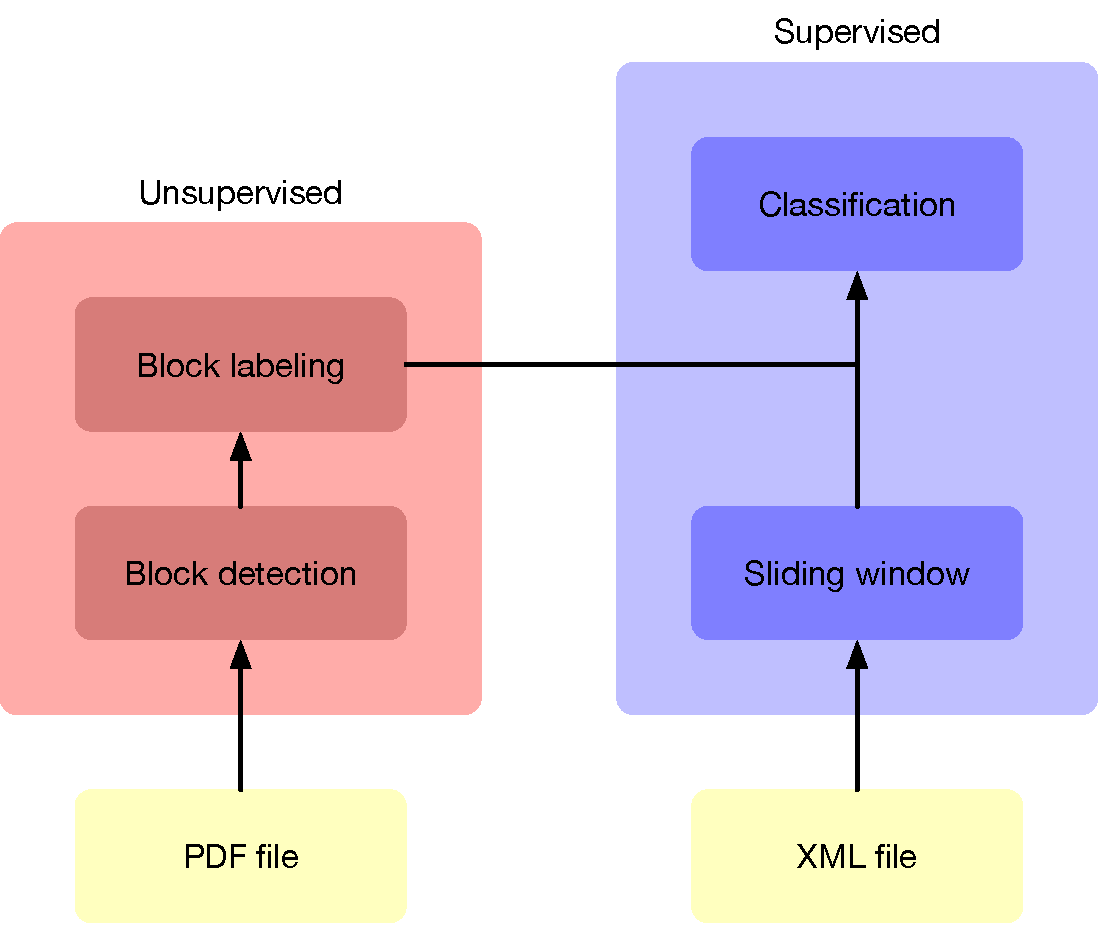
\includegraphics[width=\textwidth]{figures/layout.pdf}
  \caption{A high-level overview of the system. The unsupervised block augments
  the input to the classifier.\label{fig:overview}}
\end{figure}

\subsection{Unsupervised}%
\label{sec:unsup}
The unsupervised algorithm is inteded to detect and classify blocks of text in the
PDF file; \Cref{fig:clustered} shows an example. This approach is based on
work by \textcite{klampfl2014unsupervised}, and consists of two separate
clustering steps. First, individual characters (the fundamental objects
available in a PDF file) are clustered together into blocks of semantically
relevant text. These could be, for example,  paragraphs, section headers or page decoration.
By using the bounding boxes of the blocks, they can be clustered based on their
shape and some additional metadata (e.g.\ occurrence of font types and sizes).
The rest of this section will go into details on the two clustering steps.

\begin{figure}[tb]
  \centering
  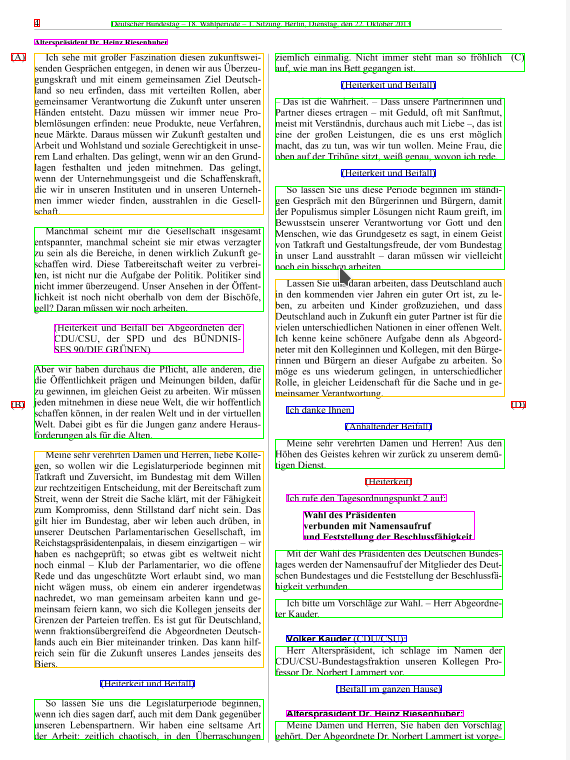
\includegraphics[height=0.5\textheight]{figures/cluster_example.png}
  \caption{An example of clustered blocks of text. Blocks with the same outline
  color belong to the same cluster.\label{fig:clustered}}
\end{figure}

\subsubsection{Hierarchical Agglomerative Clustering}
The first step is performed using hierarchical agglomerative clustering (HAC),
an unsupervised bottom-up clustering algorithm that constructs a hierarchical
tree of clusters (in this context referred to as a \emph{dendrogram}). An
example is shown in \cref{fig:hac}. The algorithm gets fed the individual
characters present in the PDF files, then iteratively groups the two closest
clusters (the initial inputs being regarded as clusters of one element) together
until only a single cluster remains. This process involves two parameters:
\begin{enumerate}
\item The distance function between two characters.
\item The distance function between two clusters of characters.
\end{enumerate}
The first parameter is trivially chosen to be the Euclidian distance between the
coordinates of the two characters. The second parameter is called the
\emph{linkage} and has several common options, the most basic of which are:
\begin{itemize}
\item Single-linkage: The distance between clusters is based on the closest two
  elements: \[ d(A, B) = \min \{ d(a, b) : a \in A, b \in B \} \]
\item Maximum-linkage: The distance between clusters is based on the furthest two
  elements: \[ d(A, B) = \max \{ d(a, b) : a \in A, b \in B \} \]
\item Average-linkage: The distance between clusters is based on the average
  distance of its elements:
  \[ d(A, B) = \frac{1}{|A||B|} \sum_{a \in A}\sum_{b \in B} d(a, b) \]
\end{itemize}
Additionally there are more involved linkage criteria, such as the Ward method
which minimizes the variance within clusters. Although these more complex
methods would generally be favored, in this specific context single-linkage
clusters is actually the best option\citep{klampfl2014unsupervised}. This is due
to its tendency to form long, thin clusters; this mirrors the nature of text, in
particular words and sentences (which are just long, thin strings of letters and
words respectively).
As an additional bonus, it is the most computationally efficient method.
While the general time complexity for HAC is
in $\mathcal{O}(n^3)$, clever algorithms exist for single-linkage clustering
that fall in $\mathcal{O}(n^2)$ \citep{sibson1973slink}, making it far more
usable on larger datasets.

\begin{figure}[tb]
  \centering
  \begin{subfigure}[b]{0.40\textwidth}
    \centering
    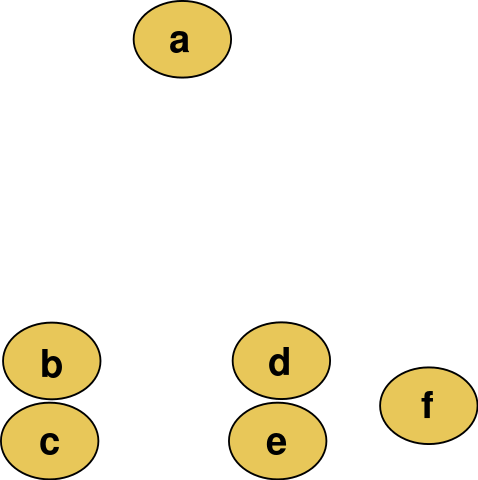
\includegraphics[width=\textwidth]{figures/dendrogram1.png}
    \caption{Before}
  \end{subfigure}
  \hspace{0.10\textwidth}
  \begin{subfigure}[b]{0.40\textwidth}
	\centering
    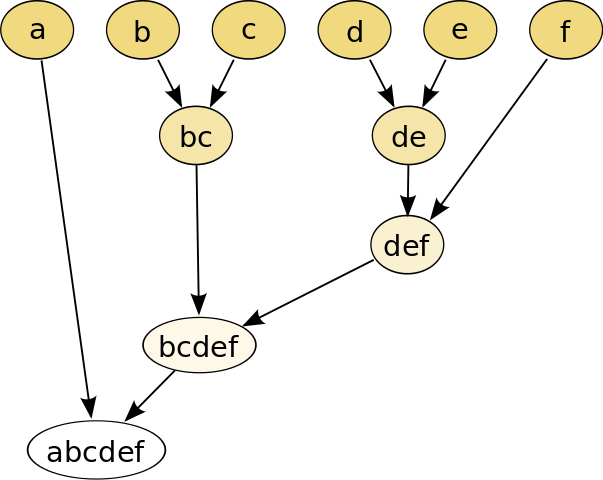
\includegraphics[width=\textwidth]{figures/dendrogram2.png}
    \caption{After}
  \end{subfigure}
  \caption{An example of hierarical agglomerative clustering, where the nodes
  are clustered by distance.\label{fig:hac}}
\end{figure}

After the dendrogram is constructed, it has to be cut at some level to obtain
the desired blocks of text. Clustering can optionally be rerun using the newly
found clusters as basic elements. This way, the document can incrementally be
clustered from characters into words, words into lines, and finally lines into
paragraphs. Both the level at which to cut the tree and the number of times to
recluster are to be manually tuned based on the particular set of documents.

\subsubsection{Clustering}
The extracted blocks from the previous step are then clustered according to
their similarity based on the following metrics:
\begin{itemize}
  \item Width of the block
  \item Height of the block
  \item The ID of the most common font occurring in the block
  \item The size of the most common font occurring in the block
\end{itemize}
This is implemented two different ways, with their performance to be compared
later on. The first method is a simple K-Means clustering, which works
as follows:
\begin{enumerate}
  \item Randomly initialize $k$ cluster centroids.
  \item Assign each observation to its nearest centroid.
  \item Recompute each centroid to be the mean of all of its assigned
    observations.
  \item Repeat steps 2 and 3 until the assignments stop changing.
\end{enumerate}
After the algorithm has converged, the clustering is defined by each
observation's nearest cluster centroid; with $k$ clusters, each observation is
assigned a $k$-dimensional one-hot vector.

\subsubsection{Dirichlet Process Clustering}

K-Means clustering can be generalized to a \emph{mixture of Gaussians} model.
Whereas K-Means clustering defines each cluster by a centroid and each
assignment by its nearest cluster, a mixture of Gaussians --- as the name
implies --- defines each cluster by a Gaussian distribution and each
assignment by a vector indicating the probabilities of belonging to each
cluster. This adds a degree of uncertainty to the representation, which is
lost in K-Means' hard assignments. While this already improves upon K-Means by
increasing the amount of information gained, it still requires a suitable
value for the number of distributions, analogous to the $K$ in K-Means
clustering. This is, at least in this case, an unintuitive parameter that
essentially has to be guessed and evaluated in order to choose a suitable
value. Luckily it can be eliminated by using an infinite mixture model. As the
name implies, an infinite mixture model is similar to a Gaussian mixture
model, except using an infinite amount of distributions, thereby removing the
most significant parameter.

The core component of this infinite mixture model is a \emph{Dirichlet
process}. This is conceptually similar to the well-known Dirichlet
distribution, with one key difference. Whereas the Dirichlet distribution
generates discrete probability distributions with a finite amount of possible
values, the Dirichlet process generates distributions with an infinite amount
of possible values. In a Dirichlet process, the proportions of how many
samples are assigned to each cluster are generated using a
\emph{stick-breaking process} (alternatively, with a \emph{P\'{o}lya urn
scheme} or a \emph{Chinese restaurant process})\citep{dirichlet}. In the
stick-breaking process, the probability $w_k$ of a sample being assigned to the
$k$'th distribution is given by
\begin{equation}
  w_k = \beta_k \cdot \prod_{i=1}^{k-1} (1 - \beta_i)\,,
\end{equation}
where $\beta_k$ is a random variable drawn from the distribution
$\mathrm{Beta}(1, \alpha)$. Since the Beta distribution is defined on the
interval $\left[0, 1\right]$, the $\beta_k$ values can be considered as
portions of a unit-length stick. When the first cluster is assigned to, a
piece of size $\beta_k$ is broken off of this unit-length stick. On subsequent
assignments, the new sample is either assigned to an existing cluster with a
probability proportional to the length of that cluster's portion of the stick,
or a new cluster is assigned to. In the latter case, the new cluster gets a
$\beta_k$-sized portion of the remains of the stick. This way, cluster
assignments tend towards a long-tailed distribution. The $\alpha$ parameter in
the prior distribution $\mathrm{Beta}(1, \alpha)$ is called the
weight- concentration parameter. As shown in \cref{fig:alpha}, the probability
mass of the distribution is inversely proportional to the value of $\alpha$.
For lower values of $\alpha$, big portions of the stick are likely to be
broken off, concentrating the cluster assignments into different clusters;
conversely, higher values of $\alpha$ lead to smaller portions and more
diversity in the cluster assignments.

\begin{figure}[tb]
  \centering
  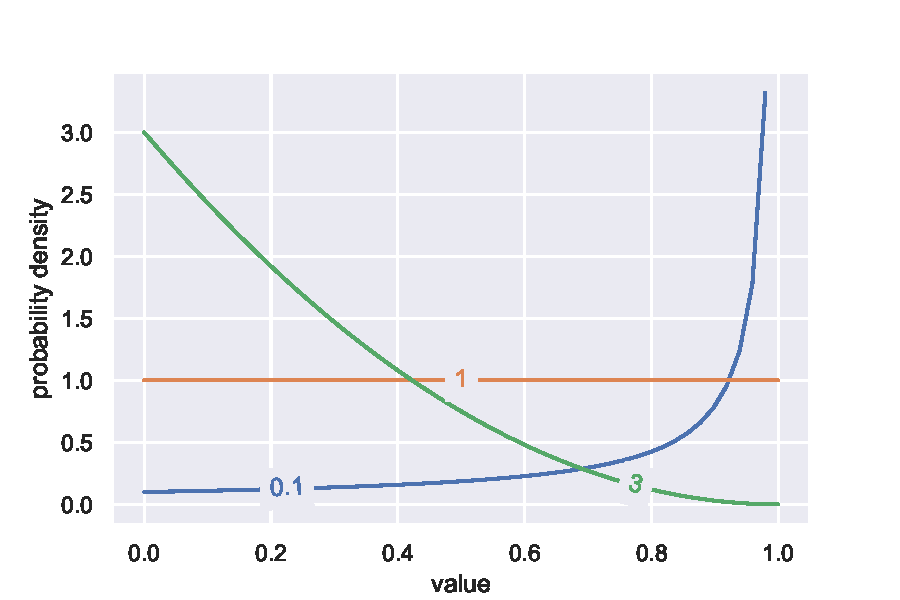
\includegraphics[width=\textwidth]{figures/alpha.pdf}
  \caption{The $\mathrm{Beta}(1, \alpha)$ distribution for various
    values of $\alpha$. As the value of $\alpha$ increases, the probability
    mass of the distribution shifts towards zero.\label{fig:alpha}}
\end{figure}

The tendency to continuously decrease the probability of assigning to a new
cluster is a key factor in using Dirichlet process clustering in practice.
Since at a certain point the probability of a new cluster being assigned
becomes practically zero, it is sufficient to implement this using a finite
``large enough'' number of clusters, after which the clusters with very low
probabilities can be pruned. This is illustrated with a simple example in
\cref{fig:gmm_example}. Note that because of the Bayesian nature of the
algorithm, even though the prior favors a long-tail distribution, it has no
problem creating equally likely clusters if the data demands it.

The samples generated from each clusters are assumed to come from a Gaussian
distribution; the rest of the probablistic model mostly consists of run-of-
the-mill priors, without much semantic meaning and differing between different
implementations of the algorithm. In this case an implementation from Scikit-
Learn\cite{scikit-learn} was used, whose probabilistic model and subsequent
derivation of the inference algorithm can be found online\footnote{http
://scikit-learn.org/stable/modules/dp-derivation.html}.

\begin{figure}[tbp]
  \centering
  \begin{subfigure}[b]{0.49\textwidth}
    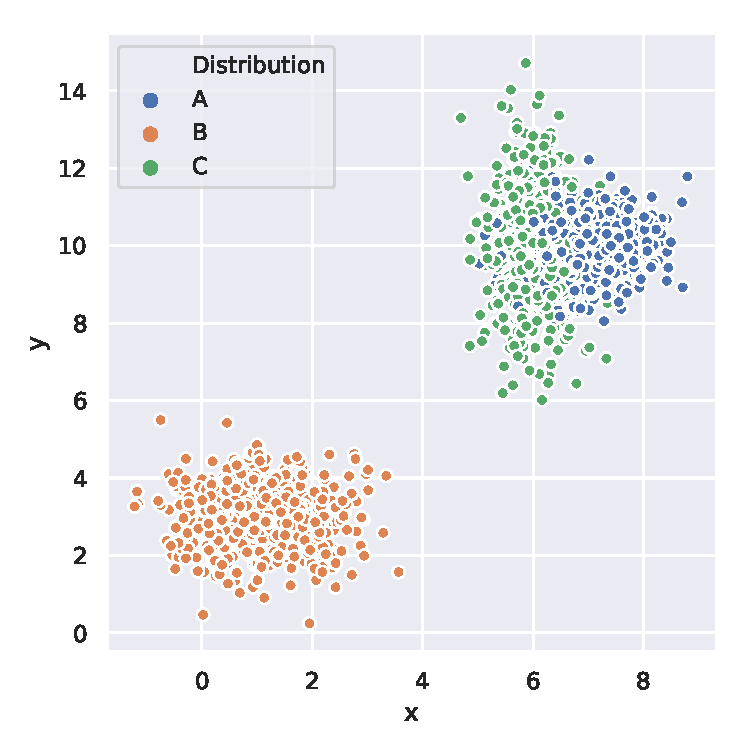
\includegraphics[width=\textwidth]{figures/clouds.pdf}
    \caption{\label{fig:gmm_cloud}}
  \end{subfigure}
  \begin{subfigure}[b]{0.49\textwidth}
    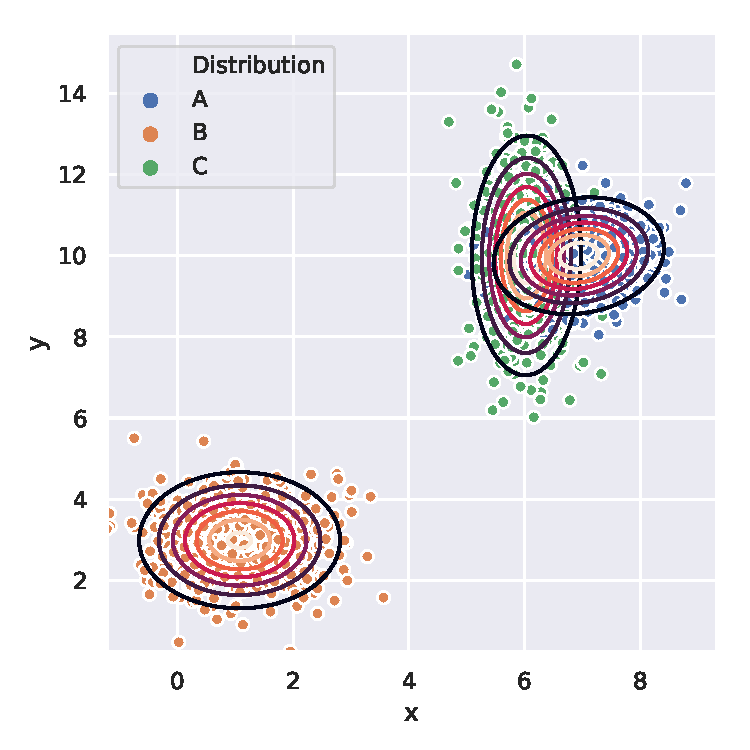
\includegraphics[width=\textwidth]{figures/gmm_dists.pdf}
    \caption{\label{fig:gmm_dist}}
  \end{subfigure}
  \begin{subfigure}[b]{0.75\textwidth}
    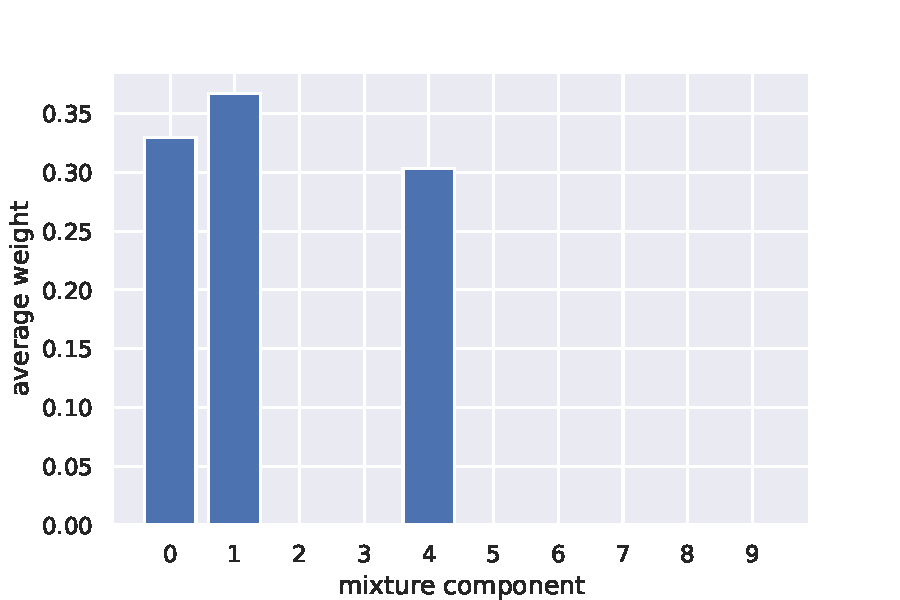
\includegraphics[width=\textwidth]{figures/gmm_assignments.pdf}
    \caption{\label{fig:gmm_ass}}
  \end{subfigure}
  % \begin{subfigure}[b]{\textwidth}
  %   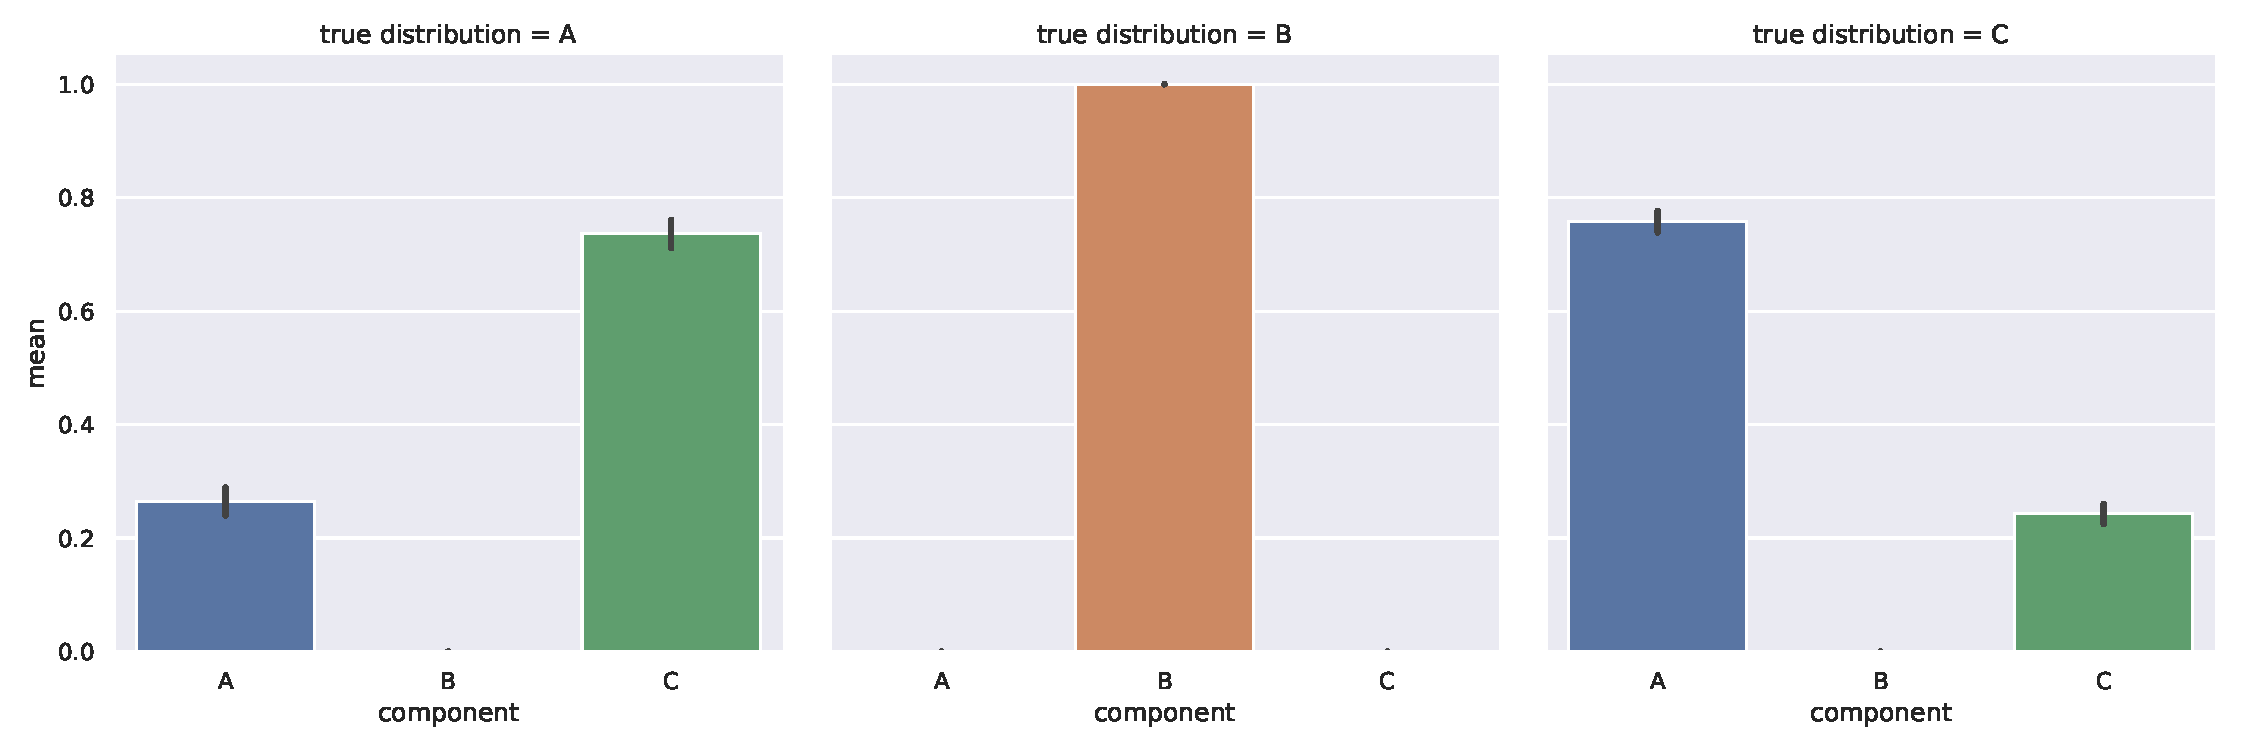
\includegraphics[width=\textwidth]{figures/gmm_skewness.pdf}
  %   \caption{d\label{fig:gmm_skew}}
  % \end{subfigure}
  \caption{Dirichlet Process mixture model clustering with a prior of 10 mixture
    components, performed on 1500 samples drawn from three different bivariate
    normal distributions (\cref{fig:gmm_cloud}). The distributions found by the
    clustering algorithm are drawn in \cref{fig:gmm_dist}. As shown by averaging
    the component weights of each sample's assignment (\cref{fig:gmm_ass}), the
    Dirichlet Process rightfully assigned to just three mixture components,
  despite its prior of ten.\label{fig:gmm_example}}
\end{figure}

\subsection{Supervised}%
\label{sec:sup}
After the data is augmented by the previously described clustering algorithms,
it's fed into a convolutional neural network for classification. Since the
documents have a dual column layout (meaning each line of text is pretty short)
and classification is based on the lines from the document, a sliding window is
used to supply more context. The window consists of a variable amount of lines
before and after the main line, which is the one supplying the label (whether
or not the line starts a new speech). This sliding window is then used as input
to a neural network, consisting of a convolutional part followed by a
fully-connected neural network part. After the convolutional part is applied to
the sliding window, the output is concatenated to the clustering distribution
obtained previously (in the case of the mixture model, this is the actual
probability distribution over each cluster; in the K-Means case, it is a
one-hot vector). There are two different models, differing in their
convolutional layer:
\begin{itemize}
  \item WordCNN: A shallow word-based architecture\citep{kim2014conv}, where the
  text is tokenized such that each token is either a word or a single punctuation
  mark (for example, ``Hello-!'' would produce the tokens ``Hello'', ``-'' and
  ``!'').
  \item CharCNN: A character-based architecture\citep{zhang2015character}. This
  is a deeper network, that operates on the raw characters without using an
  embedding layer.
\end{itemize}
The WordCNN and CharCNN models are described in \cref{tbl:wordcnn,tbl:charcnn}
; the fully-connected neural network common to both models in described in
\cref{tbl:fully_connnected}. A high-level overview of how the different parts
of the system fit together is shown in \cref{fig:overview}.

\begin{table}[tb]
  \centering
  \begin{adjustwidth}{-1cm}{-1cm}
    \begin{subtable}[t]{0.49\linewidth}
      \centering
      \begin{tabular}{rlrrr}
        \toprule
        Layer & Type & Filters & Size & Pooling \\
        \midrule
        1 & Embedding & - & 100 & - \\
        2 & Conv & 99 & $3, 5, 7$ & 1-max \\
        \bottomrule
      \end{tabular}
      \caption{The convolutional part of the WordCNN models consists of an
      embedding layer to embed the tokens into a higher-dimensional space,
      followed by a single convolutional layer. The convolutional layer
      uses 33 filters of each of three different sizes, with a stride of 1. The
      filters are concatenated for a total of 99 filters, with 1-max pooling
      applied to each filter such that the final output is a 99-dimensional vector.
      \label{tbl:wordcnn}}
    \end{subtable}
    \hspace{\fill}
    \begin{subtable}[t]{0.49\linewidth}
      \centering
      \begin{tabular}{rrrr}
        \toprule
        Layer & Filters & Size & Pooling \\
        \midrule
        1 & 256 & 7 & 3 \\
        2 & 256 & 7 & 3 \\
        3 & 256 & 3 & - \\
        4 & 256 & 3 & - \\
        5 & 256 & 3 & - \\
        6 & 256 & 3 & 3 \\
        \bottomrule
      \end{tabular}
      \caption{The convolutional part of the CharCNN model is a relatively
      deeply layered sequence of convolutions. Each convolution is followed by a
      ReLU activation function. The convolutions have a stride of 1, while the
      pooling layers are non-overlapping with a stride of 3.\label{tbl:charcnn}}
    \end{subtable}
  \end{adjustwidth}
  \vspace{1em}
  \begin{subtable}[t]{\textwidth}
    \centering
    \begin{tabular}{rrrl}
      \toprule
      Layer & Output Size & Activation & Dropout \\
      \midrule
      1 & 1024 & ReLU & Yes \\
      2 & 1024 & ReLU & Yes \\
      3 & 1 & Sigmoid & No \\
      \bottomrule
    \end{tabular}
    \caption{Both architectures go through this fully connected neural network
    with 3 layers. For the layers using dropout, a rate of 0.5 is used.
    \label{tbl:fully_connnected}}
  \end{subtable}
  \caption{The layouts of the neural networks. Table (a) corresponds to the
  convolutional part of the WordCNN model while Table (b) similarly corresponds
  to the CharCNN model; Table (c) describes the fully connected neural network
  common to both models.\label{tbl:conv_layers}}
\end{table}

The network is trained for 100 epochs, stopping early once no significant
improvement has been made on a small validation set for 10 epochs in a row.
The optimisation process is done using the Adadelta\citep{adadelta}
algorithm\footnote{Although Adam\citep{adam} has become very popular, the
architecture\citep{kim2014conv} and survey paper\citep{zhang2015conv} that
this work is based on both slightly predate the paper that popularized Adam.
Since a full analysis of different optimizers is outside the scope of this
thesis and some quick informal tests showed no difference between using
Adadelta or Adam, there is no reason to deviate from the survey.}, with binary
cross-entropy as the loss function and the training data delivered in batches
of 50 samples. Regularisation is done through a combination of
dropout\citep{dropout} and an upper limit on the L2 norm of each weight
vector\citep{l2norm}. Further explanations of the optimisation process and the
regularisation methods are provided in \cref{sec:optim} and \cref{sec:reg}
respectively.

\begin{figure}[tbp]
  \centering
  \begin{minipage}[c]{0.5\textwidth}
    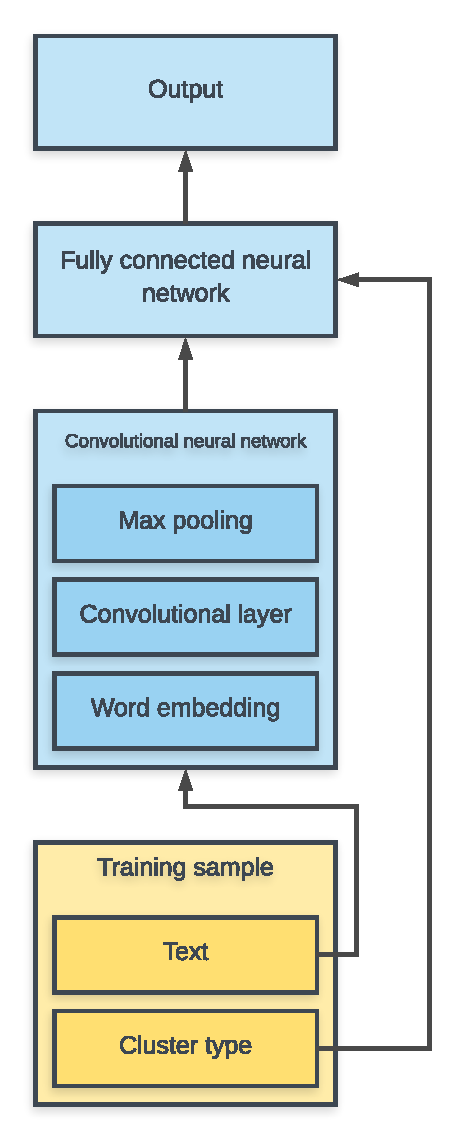
\includegraphics[width=\textwidth]{figures/nn_layout.pdf}
  \end{minipage}
  \hfill
  \begin{minipage}[c]{0.49\textwidth}
    \caption{The layout of the supervised portion of the system. The input data
    contains text and a cluster type assigned by the unsupervised portion. The
    text gets put into a convolutional neural network, the output of which is
    fed together with the cluster type into a fully connected neural network.
    The sigmoid function is applied to the output of this final neural network
    to obtain the classification.\label{fig:nn_layout}}
  \end{minipage}
\end{figure}

\subsubsection{Optimisation process}\label{sec:optim}
Optimisation is done using the Adadelta update rule\citep{adadelta}. This is
easiest to explain by starting with the basic mini-batch stochastic gradient
descent algorithm (SGD). At each iteration $t$, the network parameters $\theta$
are updated based on some calculated difference:
\begin{equation}
  \theta_{t+1} = \theta_{t} - \Delta\theta_t\,.
\end{equation}
The difference between optimization algorithms is how $\Delta\theta$ is
calculated. With SGD, it is simply
\begin{equation}
  \Delta\theta_t = \mu \loss{t}\,,
\end{equation}
where $\mathcal{L}$ is the loss function (in this case, the binary cross entropy
between the predicted labels and the true labels), and $\mu$ is an arbitrary
learning rate between 0 and 1. This learning rate is a tricky parameter to set;
too low and learning will take ages, too high and the network will fail to
converge because the steps taken are too big. One way to improve this is by
using the Adagrad\citep{adagrad} algorithm. While SGD uses a single learning
rate for the entire parameter vector, Adagrad (which stands for ``adaptive
gradient'') adapts the learning rate for each individual parameter; frequently
updated parameters get a lower learning rate, while less frequently updated
parameters are updated with a higher learning rate. This is done by simply
dividing the learning rate with the L2 norm of the sum of all previous gradients:
\begin{gather}
  g_{t} = \loss{t} \\
  \Delta\theta_t = \frac{\mu}{\sqrt{\sum^{t}_{\mathcal{T}=1}g_{\mathcal{T}}^2}} g_{t}\,.
\end{gather}
This has been found to work very well, in particular in natural language
processing and computer vision where features are often sparse, but it has two
drawbacks:
\begin{enumerate}
  \item A suitable value for the global learning rate $\mu$ has to be
    manually provided.
  \item Since the learning rate is rescaled using a monotonically increasing sum of
    previous gradient magnitudes, the learning rate will converge to zero.
\end{enumerate}
Adadelta nullifies these drawbacks by eliminating the global learning rate and
restricting the accumulation of gradients to a window of recent updates. First
of all, the sum over all previous gradients is replaced by an exponentially
decaying average of the squared gradients, referred to as $E[g^2]$:
\begin{equation}\label{eq:rms}
  E[g^2]_t = \rho E[g^2]_{t-1} + (1 - \rho) g_t^2\,.
\end{equation}
Here $\rho$ is a constant representing the rate of decay; this decaying sum
serves as a more efficient approximation of an actual window of past gradients,
which would require far more memory to store (considering both the huge number
of parameters in a neural network and the memory constraints of running on a GPU).
Substituting this into the Adagrad algorithm gives us:
\begin{align}
  \Delta\theta_t &= \frac{\mu}{\sqrt{E[g^2]_t}} g_{t} \\
		 &= \frac{\mu}{RMS[g]_t} g_{t}\,.
\end{align}
The quantity $\sqrt{E[g^2]_t}$ is called the \emph{root mean square} of $g$,
which occurs often enough in optimisation algorithms that it is often
abbreviated as $RMS[g]$. As a final step, the learning rate $\mu$ is eliminated
by replacing it with a decaying average of the previous gradient updates,
similar to \cref{eq:rms}:
\begin{equation}
  \Delta\theta_t = \frac{RMS[\theta]_{t-1}}{RMS[g]_t} g_{t}\,.
\end{equation}

\subsubsection{Regularisation}\label{sec:reg}
Dropout\citep{dropout} is a Regularisation method that is rather crude at first
glance; on each batch update, each node in the neural network has a probability
$p$ of outputting zero (i.e.\ the node being ``disabled''). As a result, nodes
cannot rely on the output of any other node being present, preventing
co-adaptation and as a result reducing the probability of overfitting on the
training data. Dropout is only active during training; when running the network
in evaluation mode, all nodes are active and the outputs are rescaled by a
factor of $1 - p$ to account for the now higher activation values.
There is another way to view dropout. It is commonly known that neural network
(or really any machine learning classifier) performance can be improved by
training a large number of them and averaging their outputs. Since every
combination of nodes disabled by dropout could be considered a unique neural
network, dropout acts as computationally cheap approximation to averaging
multiple networks.

In addition to dropout, a maximum L2 norm is imposed on each node's incoming
weight vector. If the weight vector's L2 norm exceeds this limit, it is rescaled
so that its new norm is equal to the maximum allowed norm; otherwise the weight
vector is left alone:
\begin{equation}
  \label{eq:norm}
  \vect{w} = \begin{cases}
    \vect{w}\,                          & \text{if } ||\vect{w}||^2 \leq n \\
    n \frac{\vect{w}}{||\vect{w}||^2} & \text{otherwise}
  \end{cases}
\end{equation}
This differs from the more common L2-regularisation --- where the combined L2
norm of all weight vectors is added to the loss function --- in that the weights
are not being continuously pushed towards zero, making it a milder form of
regularisation that allows for a bit more complexity in the model.

\subsubsection{Convolutional Neural Networks}\label{sec:conv}
Although convolutional neural networks (CNNs) are more closely associated with
computer vision, they are also widely used for text classification, offering
results competetive with recurrent neural networks\citep{cnnrnn} at greater
speed due to the more parallel nature of CNNs\citep{facebook}.

Convolutional neural networks (CNNs) work by taking a number of filters  of a
specified size and convolving these over the input data. A simplified example
using one filter is shown in \cref{fig:cnn}.
\begin{figure}[tb]
  \centering
  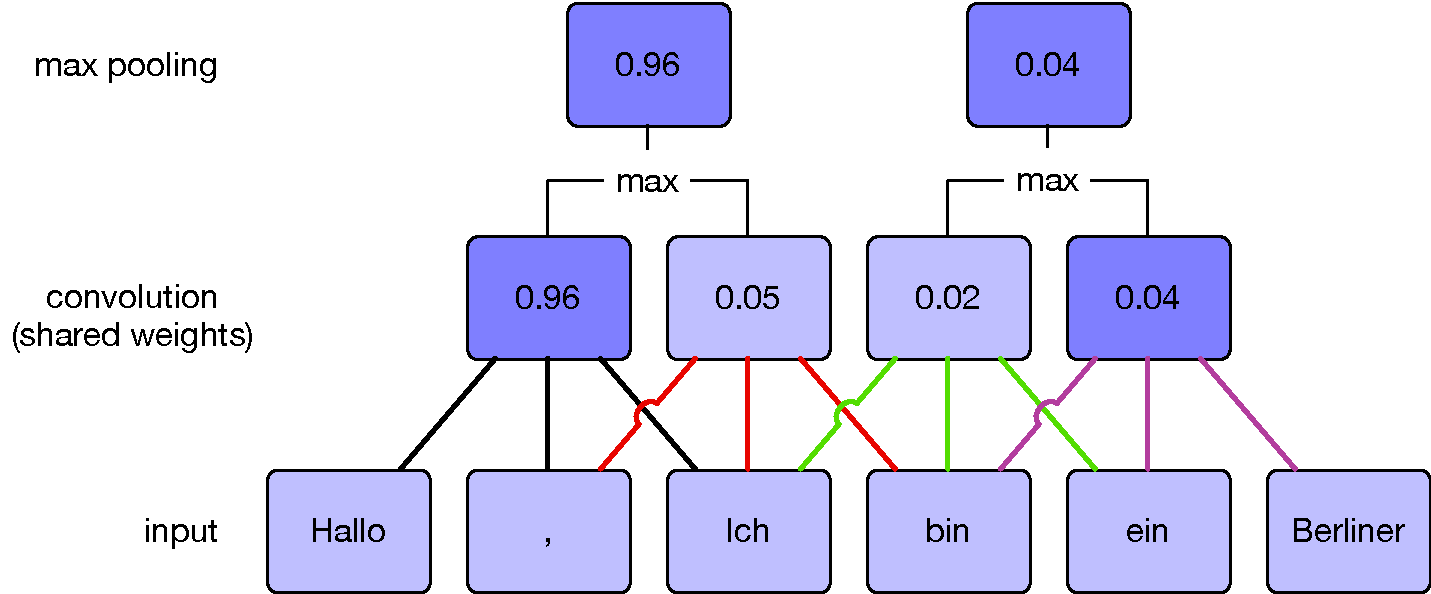
\includegraphics[width=\textwidth]{figures/cnn.pdf}
  \caption{A simplified convolutional neural network with one filter and
  max pooling.\label{fig:cnn}}
\end{figure}
In this example, the input text is convolved with a filter with a width of 3 and
a stride of 1 --- that is, each application of the filter considers three
subsequent input elements, after which the window is shifted one space to the
right. This filter is essentially a small neural network mapping three items to
one output value, whose weights are reused for each application of the filter.
Reusing the weights in this way (weight sharing) prevents the number of
parameters in the network from spiraling out of control
\citep{lecun1995convolutional}. After the application of this convolution layer,
the responses of the filter form a new sequence of roughly the same size as the
input (minus a few due to missing the edges). The next step is to downsample
this sequence by means of a \emph{max pooling} layer, which maps all values
within a window to the maximum value amongst those values. While superficially
similar to a convolution, this step generally does not involve overlap, instead
either setting the stride to the same value as the window size (usually 2) or
reducing the entire sequence to 1 value (1-max pooling). The reason for this is
twofold:
\begin{enumerate}
\item It downsamples the data, reducing the amount of parameters
  required further on in the network.
\item It adds translation invariance to the feature detected by this filter.
  The example filter of \cref{fig:cnn} reacts strongly to the first three
  words. Without the pooling layer, changing the location of these words in
  the input would similarly change the location of the high activation in the
  intermediate representation (\emph{equivariance}). The more aggressively
  the pooling is applied, the higher the degree of invariance (with full
  translational invariance being achieved with 1-max pooling).
\end{enumerate}
This combination of convolution followed by pooling can be repeated multiple
times as desired or until there is only a single value left as output from the
filter. Finally, the outputs of all filters are concatenated and fed into a
regular neural network.

While CNN architectures in computer vision are generally very deep, they tend to
be very shallow in natural language processing; commonly just a single
convolution followed by 1-max pooling \citep{zhang2015conv}.

%%% Local Variables:
%%% mode: latex
%%% TeX-master: "report"
%%% End:
